\documentclass[12pt]{article}

\usepackage{amsmath}
\usepackage{amsfonts}
\usepackage{float}
\usepackage{fancyhdr}
\usepackage{graphicx}
\usepackage[colorlinks=true,linkcolor=blue, citecolor=red]{hyperref}
\usepackage{url}
\usepackage[top=1in, left=.5in, right=.5in]{geometry}
\usepackage[utf8]{vietnam}
\usepackage{biblatex}

\addbibresource{main.bib}
\setlength{\headheight}{29.43912pt}
\addtolength{\topmargin}{-17.43912pt}

\pagestyle{fancy}
\lhead{
	Lab 02 - Phép gán và phép so sánh
}
\rhead{
    Trường Đại học Khoa học Tự nhiên - ĐHQG HCM\\
    CSC14007 - Nhập môn Phân tích độ phức tạp thuật toán
}
\lfoot{\LaTeX\ by \href{https://github.com/trhgquan}{Trần Hoàng Quân}}

\title{
	CSC14007 - Nhập môn Phân tích độ phức tạp thuật toán\\
	Lab 02 - Phép gán và phép so sánh
}
\author{Trần Hoàng Quân - MSSV: 19120338}

\begin{document}
\maketitle
\tableofcontents
\pagebreak

\section{Hướng dẫn sử dụng}
Chương trình sử dụng tập tin input \texttt{input.inp} với cấu trúc như sau:
\begin{itemize}
    \item Dòng đầu là số nguyên $t$ - số bộ test
    \item $t$ dòng tiếp theo, mỗi dòng chứa duy nhất số nguyên $n$
\end{itemize}

Chương trình sẽ output ra cửa sổ dòng lệnh $n$ dòng, dòng thứ $i$ là 3 số nguyên $f\ a\ c$ - số fibonacci thứ $n$, số lệnh gán $a$ và số lệnh so sánh $c$.
\section{Thuật toán 01 (Fibonacci đệ quy)}
\begin{figure}[H]
\centering
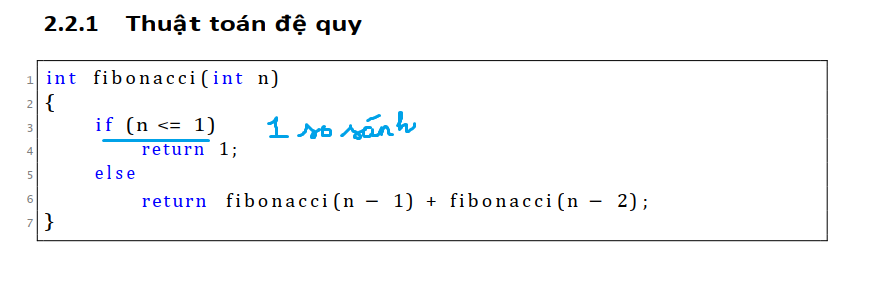
\includegraphics[]{fibo-de-quy.png}
\caption{Thuật toán Fibonacci đệ quy theo đề bài}
\end{figure}
\subsection{Phân tích thuật toán}
\subsubsection{Tổng số phép gán}
Gọi $A(n)$ là tổng số phép gán trong đoạn mã nguồn. Đoạn mã nguồn không có phép gán, vậy nên tổng số phép gán $A(n) = 0$.
\subsubsection{Tổng số phép so sánh}
Gọi $C(n)$ là tổng số phép so sánh trong toàn bộ thuật toán. Trong đoạn mã nguồn chỉ có 1 phép so sánh, tuy nhiên lại xuất hiện 2 lời gọi đệ quy. Do vậy, tổng số phép so sánh là 1 phép so sánh cộng các phép so sánh từ 2 lời gọi hàm. Ta có công thức:
$$
\begin{cases}
C(n) = 1 \text{ nếu $n \leq 1$} \\
C(n) = 1 + C(n - 1) + C(n - 2) \text{ nếu n > 1}
\end{cases}
$$
\\\\
Đây là công thức của Số Leonardo:
$$
\begin{cases}
C(n) = 1 \text{ nếu $n \leq 1$} \\
C(n) = 1 + C(n - 1) + C(n - 2) = 2F_n - 1 \text{ nếu n > 1}
\end{cases}
$$
với $F_n$ là số Fibonacci thứ $n$\cite{konuralpjournalmath848006}.

\subsection{Kiểm chứng bằng thực nghiệm}
\begin{center}
\centering
\begin{tabular}{c|c|c}
    Input $(n = ?)$ & Output lí thuyết $(F_n\ A(n)\ C(n))$ & Output thực nghiệm \\
    \hline 
    1 & 1 0 1 & 1 0 1 \\ 
    2 & 2 0 3 & 2 0 3 \\
    3 & 3 0 5 & 3 0 5 \\
    5 & 8 0 15 & 8 0 15 \\
    7 & 21 0 41 & 21 0 41 \\
    11 & 144 0 287 & 144 0 287 \\
    13 & 377 0 753 & 377 0 753 \\
    15 & 2584 0 5167 & 2584 0 5167 \\
    19 & 6765 0 13529 & 6765 0 13529 \\
    23 & 46368 0 92735 & 46368 0 92735
\end{tabular}
\end{center}

\begin{figure}[H]
\centering
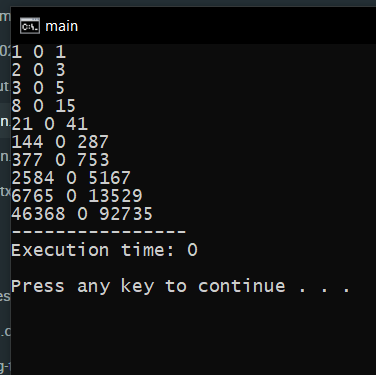
\includegraphics[]{result-de-quy.PNG}
\caption{Kết quả chạy thuật toán}
\end{figure}


\section{Thuật toán 02 (Fibonacci khử đệ quy)}
\begin{figure}[H]
\centering
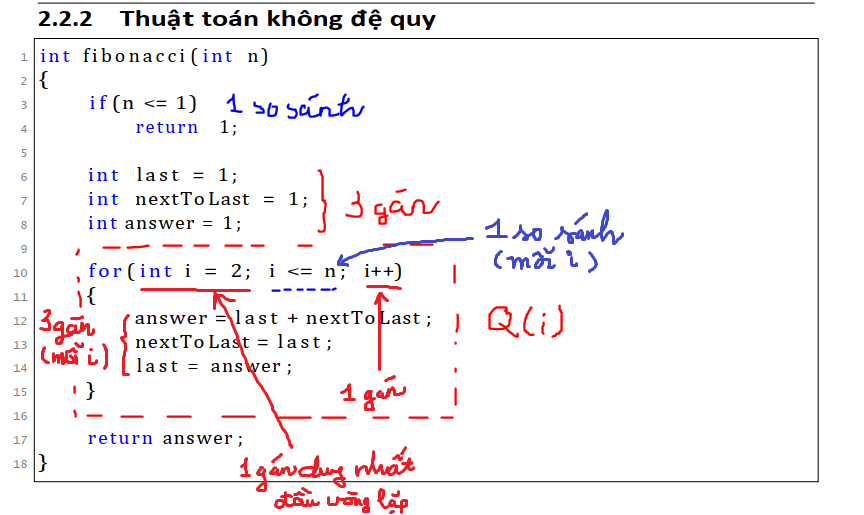
\includegraphics[scale=0.8]{fibo-khu-de-quy.png}
\caption{Thuật toán Fibonacci khử đệ quy theo đề bài}
\end{figure}

\subsection{Phân tích thuật toán}
Tiến hành phân đoạn mã nguồn như trong hình, ta có thể tính tổng số phép gán \& tổng số phép so sánh như sau:

\subsubsection{Tổng số phép gán}
Gọi $A(n)$ là tổng số phép gán trong toàn bộ thuật toán. Từ mã nguồn đã phân đoạn ta dễ dàng suy ra 
$$
\begin{cases}
A(n) = 0 \text{ nếu $n \leq 1$}\\
\displaystyle A(n) = 4 + \sum^{n}_{i = 2} Q_a(i) \text{ nếu $n > 1$}
\end{cases}
$$
với $Q_a(i)$ là số phép gán được thực hiện trong lần lặp thứ $i$.
Với $n > 1$, mỗi lần lặp có 3 lệnh gán thực hiện trong vòng \texttt{for}, 1 lệnh gán thực hiện lúc tăng biến \texttt{i++}, qua đó $\displaystyle \sum_{i = 2}^{n} Q_a(i) = \sum_{i = 2}^{n} 4 = 4(n - 1)$.
\\\\
Vậy tổng số phép gán $A(n)$ theo lí thuyết là
$$
\begin{cases}
A(n) = 0 \text{ nếu $n \leq 1$}\\
A(n) = 4 + 4(n - 1) = 4n \text{ nếu $n > 1$}
\end{cases}
$$

\subsubsection{Tổng số phép so sánh}
Gọi $C(n)$ là tổng số phép so sánh trong toàn bộ thuật toán. Từ mã nguồn đã phân đoạn ta dễ dàng suy ra
$$
\begin{cases}
C(n) = 1 \text{ nếu $n \leq 1$}\\
\displaystyle C(n) = 1 + \sum_{i = 2}^{n + 1} Q_c(i) \text{ nếu $n > 1$}
\end{cases}
$$
với $Q_c(i)$ là số phép gán được thực hiện trong lần lặp thứ $i$. Với $n > 1$, mỗi lần lặp có 1 phép so sánh thực hiện đầu vòng lặp (theo cơ chế vòng lặp $\texttt{for}$). Qua đó $\displaystyle \sum_{i = 2}^{n + 1} Q_c(i) = \sum_{i = 2}^{n + 1} 1 = n$.
\\\\
Vậy tổng số phép so sánh $C(n)$ theo lí thuyết là
$$
\begin{cases}
C(n) = 1 \text{ nếu $n \leq 1$}\\
C(n) = 1 + n \text{ nếu $n > 1$}
\end{cases}
$$
\subsection{Kiểm chứng bằng thực nghiệm}
\begin{center}
\centering
\begin{tabular}{c|c|c}
    Input $(n = ?)$ & Output lí thuyết $(F_n\ A(n)\ C(n))$ & Output thực nghiệm \\
    \hline 
    1 & 1 0 1 & 1 0 1 \\ 
    2 & 2 8 3 & 2 8 3 \\
    3 & 3 12 4 & 3 12 4 \\
    5 & 8 20 6 & 8 20 6 \\
    7 & 21 28 8 & 21 28 8 \\
    11 & 144 44 12 & 144 44 12 \\
    13 & 377 52 14 & 377 52 14 \\
    15 & 2584 68 18 & 2584 68 18 \\
    19 & 6765 76 20 & 6765 76 20 \\
    23 & 46368 92 24 & 46368 92 24
\end{tabular}
\end{center}

\begin{figure}[H]
\centering
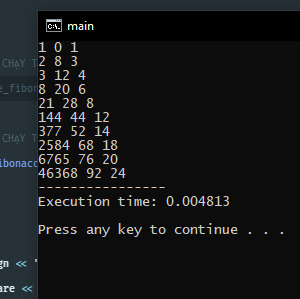
\includegraphics[]{result-khu-de-quy.PNG}
\caption{Kết quả chạy thuật toán}
\end{figure}

\printbibliography
\end{document}